\chapter{Estruturas de um Sistema RAV}
Os conceitos e definições necessárias para o desenvolvimento deste trabalho, foram apresentados nos capítulos anteriores, neste capítulo será apresentando toda a estrutura para implementação do sistema de reconhecimento de voz.

O sistema RAV proposto, foi implementado para um sistema independente do locutor, visando um jogo divertido para o maior número de pessoas possíveis, com o modo de pronúncia de palavras isoladas, e um vocabulário pequeno, que faz parte de um diciónario pré-definido. 

Este sistema foi desenvolvido em Java, com suas Apis e direcionada para sistemas operacionais Android, tendo como base a teoria dos Modelos Ocultos de Markov para o modelamento de sequencias de frames. Então cada elocução é dividida em quadros de tempos com iguais durações, extraindo seus parâmetros de cada um deles para se criar os modelos Hmms para cada palavra do dicionário, como sistemas de reconhecimento de palavras isoladas necessitam da captura do início e fim das palavras pronunciadas, o usuário deve pronunciar um comando, e depois de um breve intervalo, pronunciar o próximo, os comandos disponíveis no dicionário da aplicação são: “Direita”, “Esquerda”, “Acima” e “Abaixo”. O personagem do jogo só responderá ao comando dito, depois de reconhecer qual é o comando falado, em caso de sucesso, o jogo continua normalmente, até a vitória ou derrota do jogador, em caso do não reconhecimento da palavra, o sistema ignora a palavra dita. Outra característica importante do reconhecedor é a tentativa de capturar o humor do jogador com palavras ofensivas gravadas no dicionário, o sistema apresenta uma penalidade em caso dessas palavras serem pronunciadas.

Este trabalho pode ser dividido em 6 etapas: Aquisição da fala, Pré-Processamento, Extração de Parâmetros, Criação de referências, Classificação e Execução dos comandos.

\section{Arquitetura de um sistema RAV}
O sistema RAV pode ser definido em 4 processos que são mostrados na figura \ref{figArqRav}, esses processos são compostos por outras etapas. O primeiro processo da figura \ref{figArqRav} é chamado de \textit{Front-End}, que engloba as etapas de captura do sinal da fala, conversão do sinal elétrico em sinal analógico-digital e o processo de filtragem. Outro processo ilustrado na figura \ref{figArqRav} é o \textit{Modelo Acústico} que é a fase responsável pelo treinamento das unidades a serem reconhecidas. O \textit{Reconhecedor} é a parte que une todas os processos, é onde é feito as comparações entre o sinal falado e filtrado com os padrões de referência, que fazem parte da gramática adotada no sistema, o processo \textit{Gramática} contém o dicionário de modelos da aplicação. 

\begin{figure}[H]
\includegraphics[width=1\textwidth]{graficos/desenvolvimento_rav.eps}
\caption{Diagrama de Atividades do Sistema}
\label{figArqRav}
\end{figure}

Com resultado da transcrição, são executados os comandos do jogo, no dispositivo móvel.

\subsection{Front-End}
Nesta seção serão mostrados os processos necessários para etapa \textit{Front-End}, que são: \textit{Aquisição de fala} junto com a \textit{conversão analógico-digital} e o \textit{Processo de filtragem} que também é chamado de pré-processo.

\begin{enumerate}[A)]
\item {Aquisição da fala:}

A interação do usuário com a aplicação é feita apenas com a voz, ao iniciar o sistema, a interface de voz com usuário é habilitada, permitindo ao usuário interagir com os comandos definidos no vocabulário. Como a aplicação é destinada a dispositivos móveis, a captura do som, é feita pelo microfone do celular ou tablet, fornecendo um sinal elétrico, sendo nessário uma filtragem do sinal analógico resultante por um filtro passa-baixas, chamado de anti-aliasing, para depois ser feita a conversão analógio-digital \cite{DigitalProcRabiner}. Esse filtro tem o intuito de suprimir componentes de frequência superiores à metade da frequência de amostragem, sendo chamado de Nyquist \cite{DigitalSigProakis}.

A última etapa da aquisição da fala é a conversão do sinal de fala analógico em digital através de um
amostrador, possibilitando o processamento digital. Segundo \citeonline{PattRecChou} é nesta fase que são
escolhidas a taxa de amostragem, impossibilitando a ocorrência do efeito de aliasing e a precisão usada para a gravação do sinal, a partir do número de níveis que esse sinal poderá assumir. 
Todas etapas podem ser vistas na subseção \ref{subsec:fala} deste trabalho.

\item {Pré-Processamento:}

Sistemas RAV sofrem com características do ambiente de gravação e o canal de comunicação, como ruídos de alta frequência, distância do microfone, períodos de silêncio, etc. Uma forma de amenizar esse proplemas é fazer o sinal passar por um processo chamado de pré-processamento, deixando o sinal mais próximo da fala pura. As etapas desse processo podem ser mostradas na figura 7 \cite{RavIsolAnderson}. 

\begin{figure}[H]
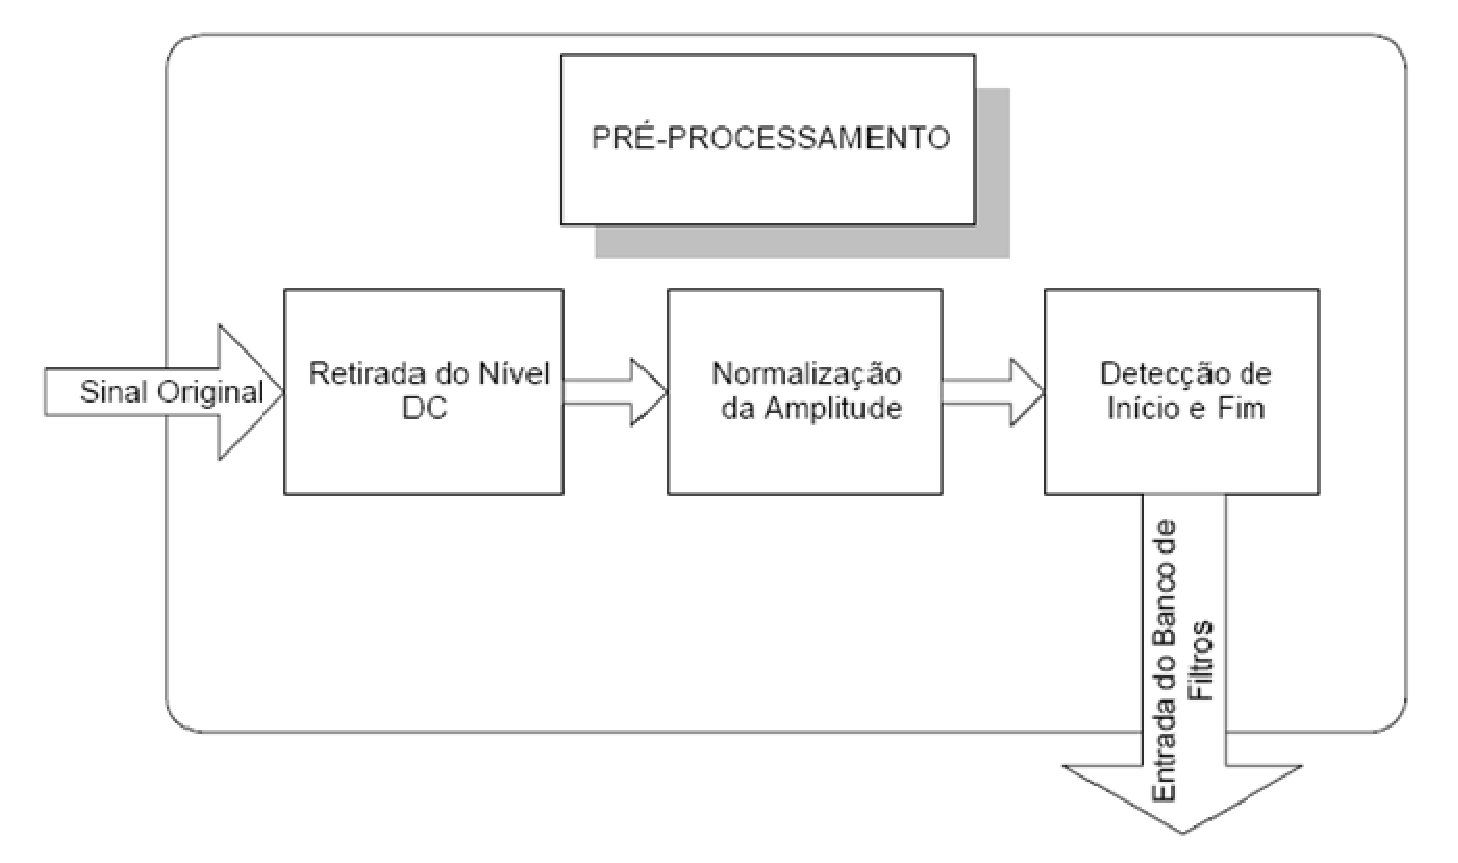
\includegraphics[width=0.8\textwidth]{graficos/pre_proc.eps}
\caption{Diagrama de blocos da fase de pré-processamento}
\end{figure}

Calculando a média aritmétrica das amplitudes do sinal digital e subtraindo de cada aplitude esta média, consegue-se retirar o nível DC, que é uma componente contínua que atrapalha a comparação em valores absolutos. Outro problema encontrado é o diferencial entre sons mais baixos e sons mais altos, que é resolvido com a normalização da amplitude, esse pré-processamento do sinal faz com que todos os valores de amplitude de todos os sinais estejam na faixa de -1 e 1, garantindo que esses sinais sejam processados igualmente no algoritmo de reconhecimento. Esse processo é possível dividindo o valor de cada amostra do sinal pelo maior valor de aplitude do mesmo. 

A última fase do pré-processamento no sistema RAV de palavras isoladas é a detecção do início e fim da locução, a fim de remover de forma precisa períodos de silêncio, que podem conter ruídos, sinais indesejados e a duração do sinal falado \cite{RavIsolAnderson}. De acordo com \citeonline{SpeechCodChu} esse processo também tem como objetivo diminuir a carga computacional e economizar tempo, já que o sistema poderá processar apenas trechos que fazem parte da fala.
 O extremo inicial é determinado pelo primeiro quadro onde realmente se inicia a fala e o extremo final é
determinado pelo último quadro que ainda há fala.
\end{enumerate}

\subsection{Modelo Acústico}
Processo que define as unidades a serem modeladas, extração de parâmetros e modelos ocultos de markov se encaixam nessa fase do processo.

\begin{enumerate}[A)]
\item Extração de Parâmetros:

A extração de parâmetros é uma etapa de grande importância em um sistema RAV, pois o sinal digital possui uma grande quantidade de dados e uma análise direta necessitaria tempo e processamento consideráveis e ainda sim, não apresentariam um resultado expressivo. Muitas informações existentes no sinal digital puro não possuem significância alguma para a distinção fonética, assim o classificador empregado dificilmente conseguirá diferenciar amostras de palavras distintas.

No trabalho de \citeonline{RavIsolAnderson} é mostrado a idéia básica da extração de parâmetros, que é representar segmentos, fonemas ou qualquer outra unidade de fala com o menor número possível de parâmetros, com informações necessárias para caracterizar o sinal de fala. Por melhor que seja o classificador, este só apresentará bons resultados se os parâmetros utilizados durante o treinamento ou reconhecimento contiverem informações relevantes. Uma redução no volume de dados mantendo informações suficientes para a caracterização do sinal viabilizará uma classificação robusta e confiável.

Algumas técnicas de análise espectral são mostradas por \citeonline{DigitalProcRabiner} e são usadas para obter os parâmetros do sinal digital, elas são: a transformada rápida de Fourier (Fast Fourier Transform ou FFT), os métodos de banco de filtros (Filter Bank), os de análise homomórfica ou análise cepstral (mel-cepstrum) e os de codificação por
predição linear (Linear Predictive Coding ou LPC).

A técnica FFT, os métodos de banco de filtros e o LPC foram muito utilizados para a análise espectral da fala, no entanto, elas possuem algumas restrições, por isso \citeonline{DiscreteDeller} propõe o uso da técnica \textit{mel-cepstrum}, cujo os coeficientes mel-cepstrais (Mel-Frequency Cepstral Coefficients ou MFCC), são obtidos pela representação em freqüência na escala \textit{Mel}, a que considera a técnica mais apropriada para ser
utilizada no processo de reconhecimento de voz. Com vantagens no uso dessa técnica, atualmente os coeficientes MFCC
são os mais populares \cite{IsolatWordBouroba}.
\item Treinamento dos Modelos Ocultos de Markov:

A fase de treinamento é uma das etapas de maior importancia em um sistema de reconhecimento de voz independente do locutor e ser o fator determinante na obtenção de um sistema com bons resultados ou não. É o momento em que são definidos os modelos HMMs para cada palavra do vocabulário utilizado.

A definição da quantidade de estados necessários para modelar uma palavra e o número de misturas por estado não são definidos por uma regra, mas sim, dependente da familiaridade com os modelos HMMs ou por intuição, além de serem necessários muitos testes para obtenção do melhor resultado. 
%Escrever a quantidade de estados e misturas no momento da implentação
\end{enumerate}

\subsection{Reconhecedor}
Pode ser considerado a central do sistema RAV, é a etapa que une todas os outros processos e define o resultado de sucesso ou fracasso do reconhecimento.

\begin{enumerate}[A)]
\item Reconhecimento:

Como citado em \citeonline{RavIsolAnderson} a fase de reconhecimento consiste em dada uma elocução, descobrir qual o modelo que tem a maior probabilidade de gerá-la. Nesta etapa é necessário apenas o pré-processamento e da extração de características que gera a sequência de observações a ser utilizada no algoritmo de reconhecimento. O procedimento de
reconhecimento pode ser visualizado na figura baseada em \cite{TutorialHmmRabiner}.

\begin{figure}[H]
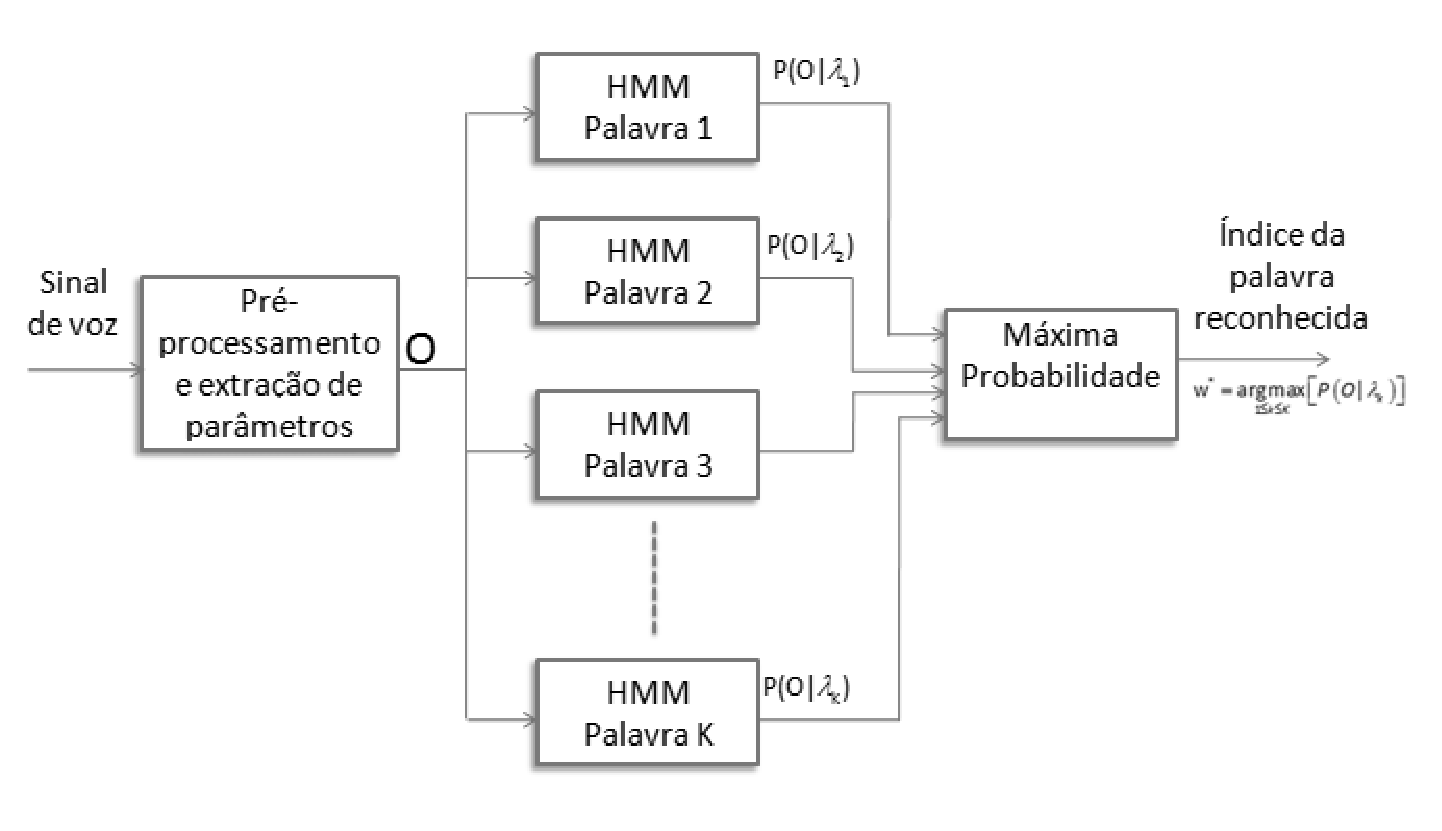
\includegraphics[width=0.9\textwidth]{graficos/reconhecimento.eps}
\caption{Procedimento de reconhecimento}
\end{figure}

O algoritmo \textit{forward} pode ser usado para o reconhecimento a fim de se determinar a probabilidade de cada modelo de palavra gerar uma dada elocução. O modelo com maior probabilidade é o escolhido como correspondente à palavra falada, assumindo que todas as palavras têm uma mesma probabilidade de ocorrência. O algoritmo de \textit{Viterbi} também pode ser utilizado para esta classificação, embora este resulte apenas em uma aproximação
para a probabilidade de uma dada sequência de observações. Os resultados utilizando-se um ou outro algoritmo são praticamente idênticos \cite{RavIsolAnderson}.
\end{enumerate}

\subsection{Gramática}
As unidades treinadas que serão modelos do reconhecimento são consideradas a gramática do sistema.

\begin{enumerate}[A)]
\item Construção do dicionário de códigos:

Também chamado de codeblock  é gerado a partir da base de dados de treinamento seguindo um critério de otimização. \citeonline{AnAlgorLinde} propos um algoritmo muito eficiente para o treinamento, conhecido como algoritmo LBG. No caso do reconhecimento de voz para palavras isoladas, cada elocução é dividida em vetores (frames) com os parâmetros obtidos. Para cada um dos modelos HMM, todos os frames de cada elocução da palavra que ele
representa são distribuídos entre todos os estados do mesmo de maneira uniforme. Após esta divisão calcula-se para cada estado um vetor centróide a partir de todos os vetores pertencentes a este estado \cite{RavIsolAnderson}.
\end{enumerate}
